\documentclass[11pt,jou]{apa6}
\usepackage{apacite}
\usepackage{graphicx}
\usepackage{pdfsync}
\usepackage{hyphenat}
\usepackage{verbatim}
\usepackage{multirow}
\usepackage{rotating}
\usepackage{color,soul}

% typeface command
\tolerance=500

% Prevent breaking inline formulae
\relpenalty=9999
\binoppenalty=9999



\title{Learning to compete}
\shorttitle{Learning to compete}
\author{.}
\affiliation{.}
\leftheader{.}
%\abstract{.}
%\keywords{.}

%\authornote{Brian D. Beitzel, Department of Educational Psychology,
%  Counseling and Special Education, SUNY Oneonta.
%
%  Correspondence concerning this article should be addressed to Brian
%  D. Beitzel, Department of Educational Psychology, Counseling and
%  Special Education, SUNY Oneonta, 129 Fitzelle Hall, Oneonta, NY
%  13820.  E-mail: beitzebd@oneonta.edu}

\begin{document}
\maketitle




\section{Competition in decisions from experience}

\cite{phillips2014rivals}

\section{Experiment 1}

\subsection{Participants and materials}

\hl{X} participants were recruited through Amazon Mechanical Turk (www.mturk.com) using \emph{psiTurk}.
Participants were paid a base payment of \$.50 for their participation, as well as a bonus of up to \$3 depending on their performance.

\subsection{Procedure}

\begin{figure*}[ht]
\centerline{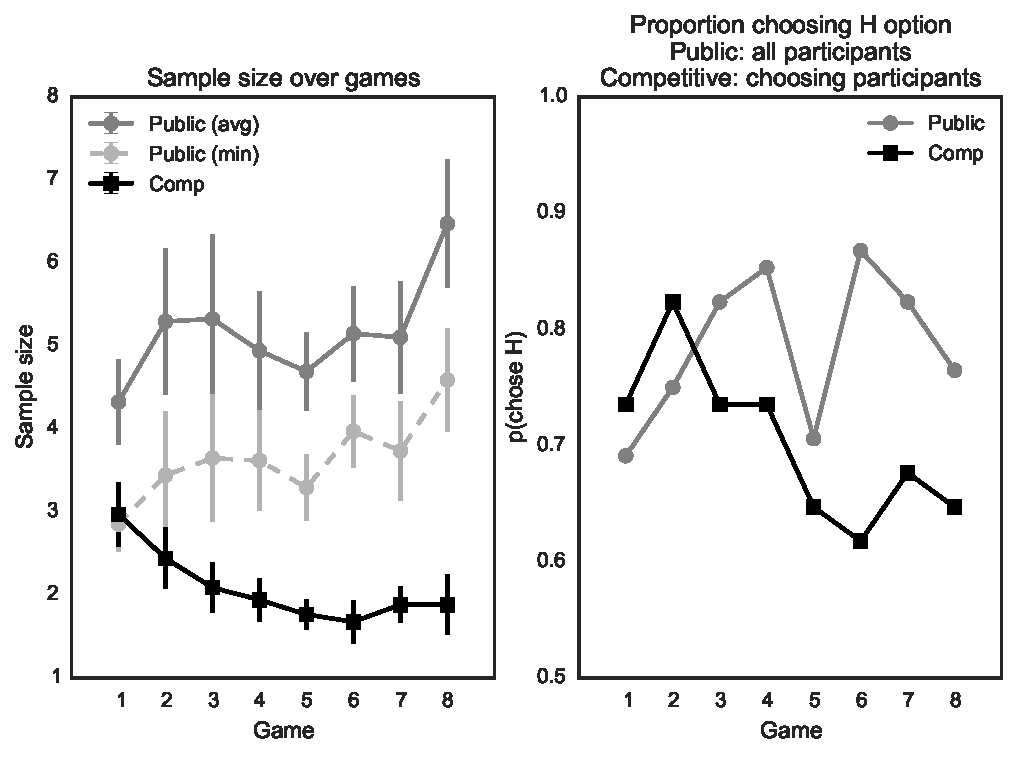
\includegraphics[width=4in]{figures/exp1_results.pdf}}
\caption{Caption}
\label{exp1_results.fig}
\end{figure*}

\subsubsection{Option environment}

Each decision problem involved two options $H$ and $L$ with higher and lower expected value, respectively.
Each option was associated with two possible outcomes: a \emph{common} outcome that occurred with probability $p = .8$ and a \emph{rare} outcome that occurred with probability $1 - p = .2$.
For each option, the common outcome was a random number in the range $[-20, 20]$, while the rare outcome was a random number in the range $[-200, 200]$.
Option sets were randomly generated and retained if the difference between the expected value for the $H$ and $L$ options was greater than or equal to $25$. 
Twenty problem sets comprised of 8 problems each were generated with this procedure.
Problem sets were resampled if the summed expected value across all $L$ options was less than $-100$ or the summed expected value of all $H$ options was greater than $200$, ensuring that each participant's total payoff would lie in that range.

Participants were told about the option structure, including the relative probabilities of the common and rare outcomes.
Prior to playing any games, they completed four trials of non-consequential sampling with individual options.
For each option, they were instructed to sample 25 time and observing the resulting outcome.
They then reported the highest and lowest outcomes that were seen during sampling, and estimated the expected value of the option.
All participants experienced the same four example options, which were chosen to include options where both outcomes were in the same domain (i.e., both the common and rare outcome were gains) and options where they were in different domains (i.e., a common loss but rare gain with high value).
This training ensured that participants had experience with the structure of individual options prior to the game, including the relative frequency and range of each outcome type. 
In addition, it served as an \hl{instructional check to evaluate whether participants were able to report both outcomes they observed during sampling}.\footnote{any participants excluded based on this?}

Participants were endowed with an initial bonus of \$1.00 at the beginning of the experiment, and were instructed that their payoff from each game (the expected value of the the option they selected) would be added or subtracted when determining their final bonus.

\subsubsection{Group formation and coordination}

After completing the instructions, participants were presented with a list of open groups.
After joining an open group, they waited for a second participant to join the same group. 
When the group was full, both participants then confirmed that they were ready to play.
This confirmation was required for the experiment to begin to ensure that both players were present and attending to the experiment.

The experiment was designed such that the game advanced only when decisions were received from both players and broadcast to the entire group. 
For example, each game started when both participants confirmed they were ready to begin.
Similarly, during the sampling phase, players continued to the next trial when they received their opponent's decision to either stop or continue sampling.

\subsubsection{Gameplay}

On each sampling trial, a participant clicked on one of the two options and observed a randomly generated outcome (in the form of a coin labeled with the number of points between -200 and 200). 
The outcome remained visible until the participant indicated if they wanted to 1) ``Continue learning" or 2) ``Stop and choose". 
If both players decided to continue sampling the experiment proceeded to the next sampling trial.

If one player decided to choose an option, they then clicked on one of the two options to claim it. 
When an opponent claimed an option, an icon appeared on the other player's display indicating the choice. 
If both players decided to stop on the same trial, a random choice order was generated which determined which participant went first.

\subsubsection{Public condition}

In the public condition, a player's choices were shared with their opponent but had no other consequence in terms of their ability to sample or choose.
When a player decided to stop, their selection was visible to their opponent in the form of a gray person symbol that appeared below the option they chose. 
However, the opponent could continue sampling for as many turns as they desired, and when they stopped could select either of the two options.
Both players were still required to acknowledge the outcome of every turn (i.e., how many players chose an option), ensuring that a player who stopped was still paying attention for the remainder of the game.




\subsubsection{Competitive condition}

In the competitive condition, one player's decision to stop and claim an option had the effect of removing it from the set of options available to their opponent.
When such a choice occurred, the option faded out on the display and the opponent was required to select the remaining option (thus, they were not permitted to continue sampling).
All other aspects of the gameplay were the same as in the public condition.

\subsubsection{Feedback}

There was no feedback on individual games.
At the end of the experiment, participants were informed as to the expected value of the options they had selected and their total bonus.



\subsection{Results}




\subsubsection{Sample size}

Sample size was greater in the public condition than in the competitive condition. No change in sample size in the public condition over games. Decline in sample size in the competitive condition across games.

Increase in ties over games in the competitive condition, indicating convergence of strategies.

The decrease in sample size at the group level was evident at the level of individual pairs, with 23 pairs (68\%) in the competitive condition showing a decrease in average sample size from the first half to second half of the experiment. Of the remaining pairs, 5 (15\%) showed no change, and 6 (18\%) showed an increase in average sample size.
In comparison, participants in the public condition showed the opposite pattern of change from first to second halves of the experiment, with 21 (31\%) showing a decrease, 5 (7\%) showing no change, and 42 (62\%) showing an increase.


\subsubsection{Performance}

Did the person receiving do worse than the person choosing in the competitive condition? The interesting thing would be if that is NOT the case -- that the increased competition didn't actually make people better off.

Show proportion choosing the better option in Public (first), Public (second), Competitive (chooser), Competitive (receiver).

\subsection{Discussion}

Interesting to note that this change in the competitive condition occurred in the absence of any feedback.\footnote{Of course, there is some feedback in the sense that people may have a preference regarding the two options, and they can observe an opponent's choice with respect to their own preferences. That is, can experience an opponent taking an option that seemed better or that one was learning about.}
Results in the public condition suggest that the effect is not due to further learning about the option environment, since the level of sampling was sustained in that condition across games.
Thus, we conclude that participants adjusted their sample size in response to observing a competitor choose first.


\section{Experiment 2}

Role of no, partial, and full feedback.



\section{Experiment 3}


\bibliographystyle{apacite}
\bibliography{library}
\end{document}
